% !TEX encoding = UTF-8 Unicode

\documentclass[9pt, openany]{extbook}
\usepackage{Genesys}
\usepackage{hyperref}
\geometry{papersize={5.5in, 8.5in}}
\usepackage{wrapfig}
\graphicspath{{img/}}
\newfontfamily\TF{Gemina 2 Regular}
\setcounter{tocdepth}{1}


\usepackage{eso-pic}

\newcommand\BackgroundPic{%
\hspace*{-0.2\paperwidth}
\parbox[b][\paperheight]{\paperwidth}{%
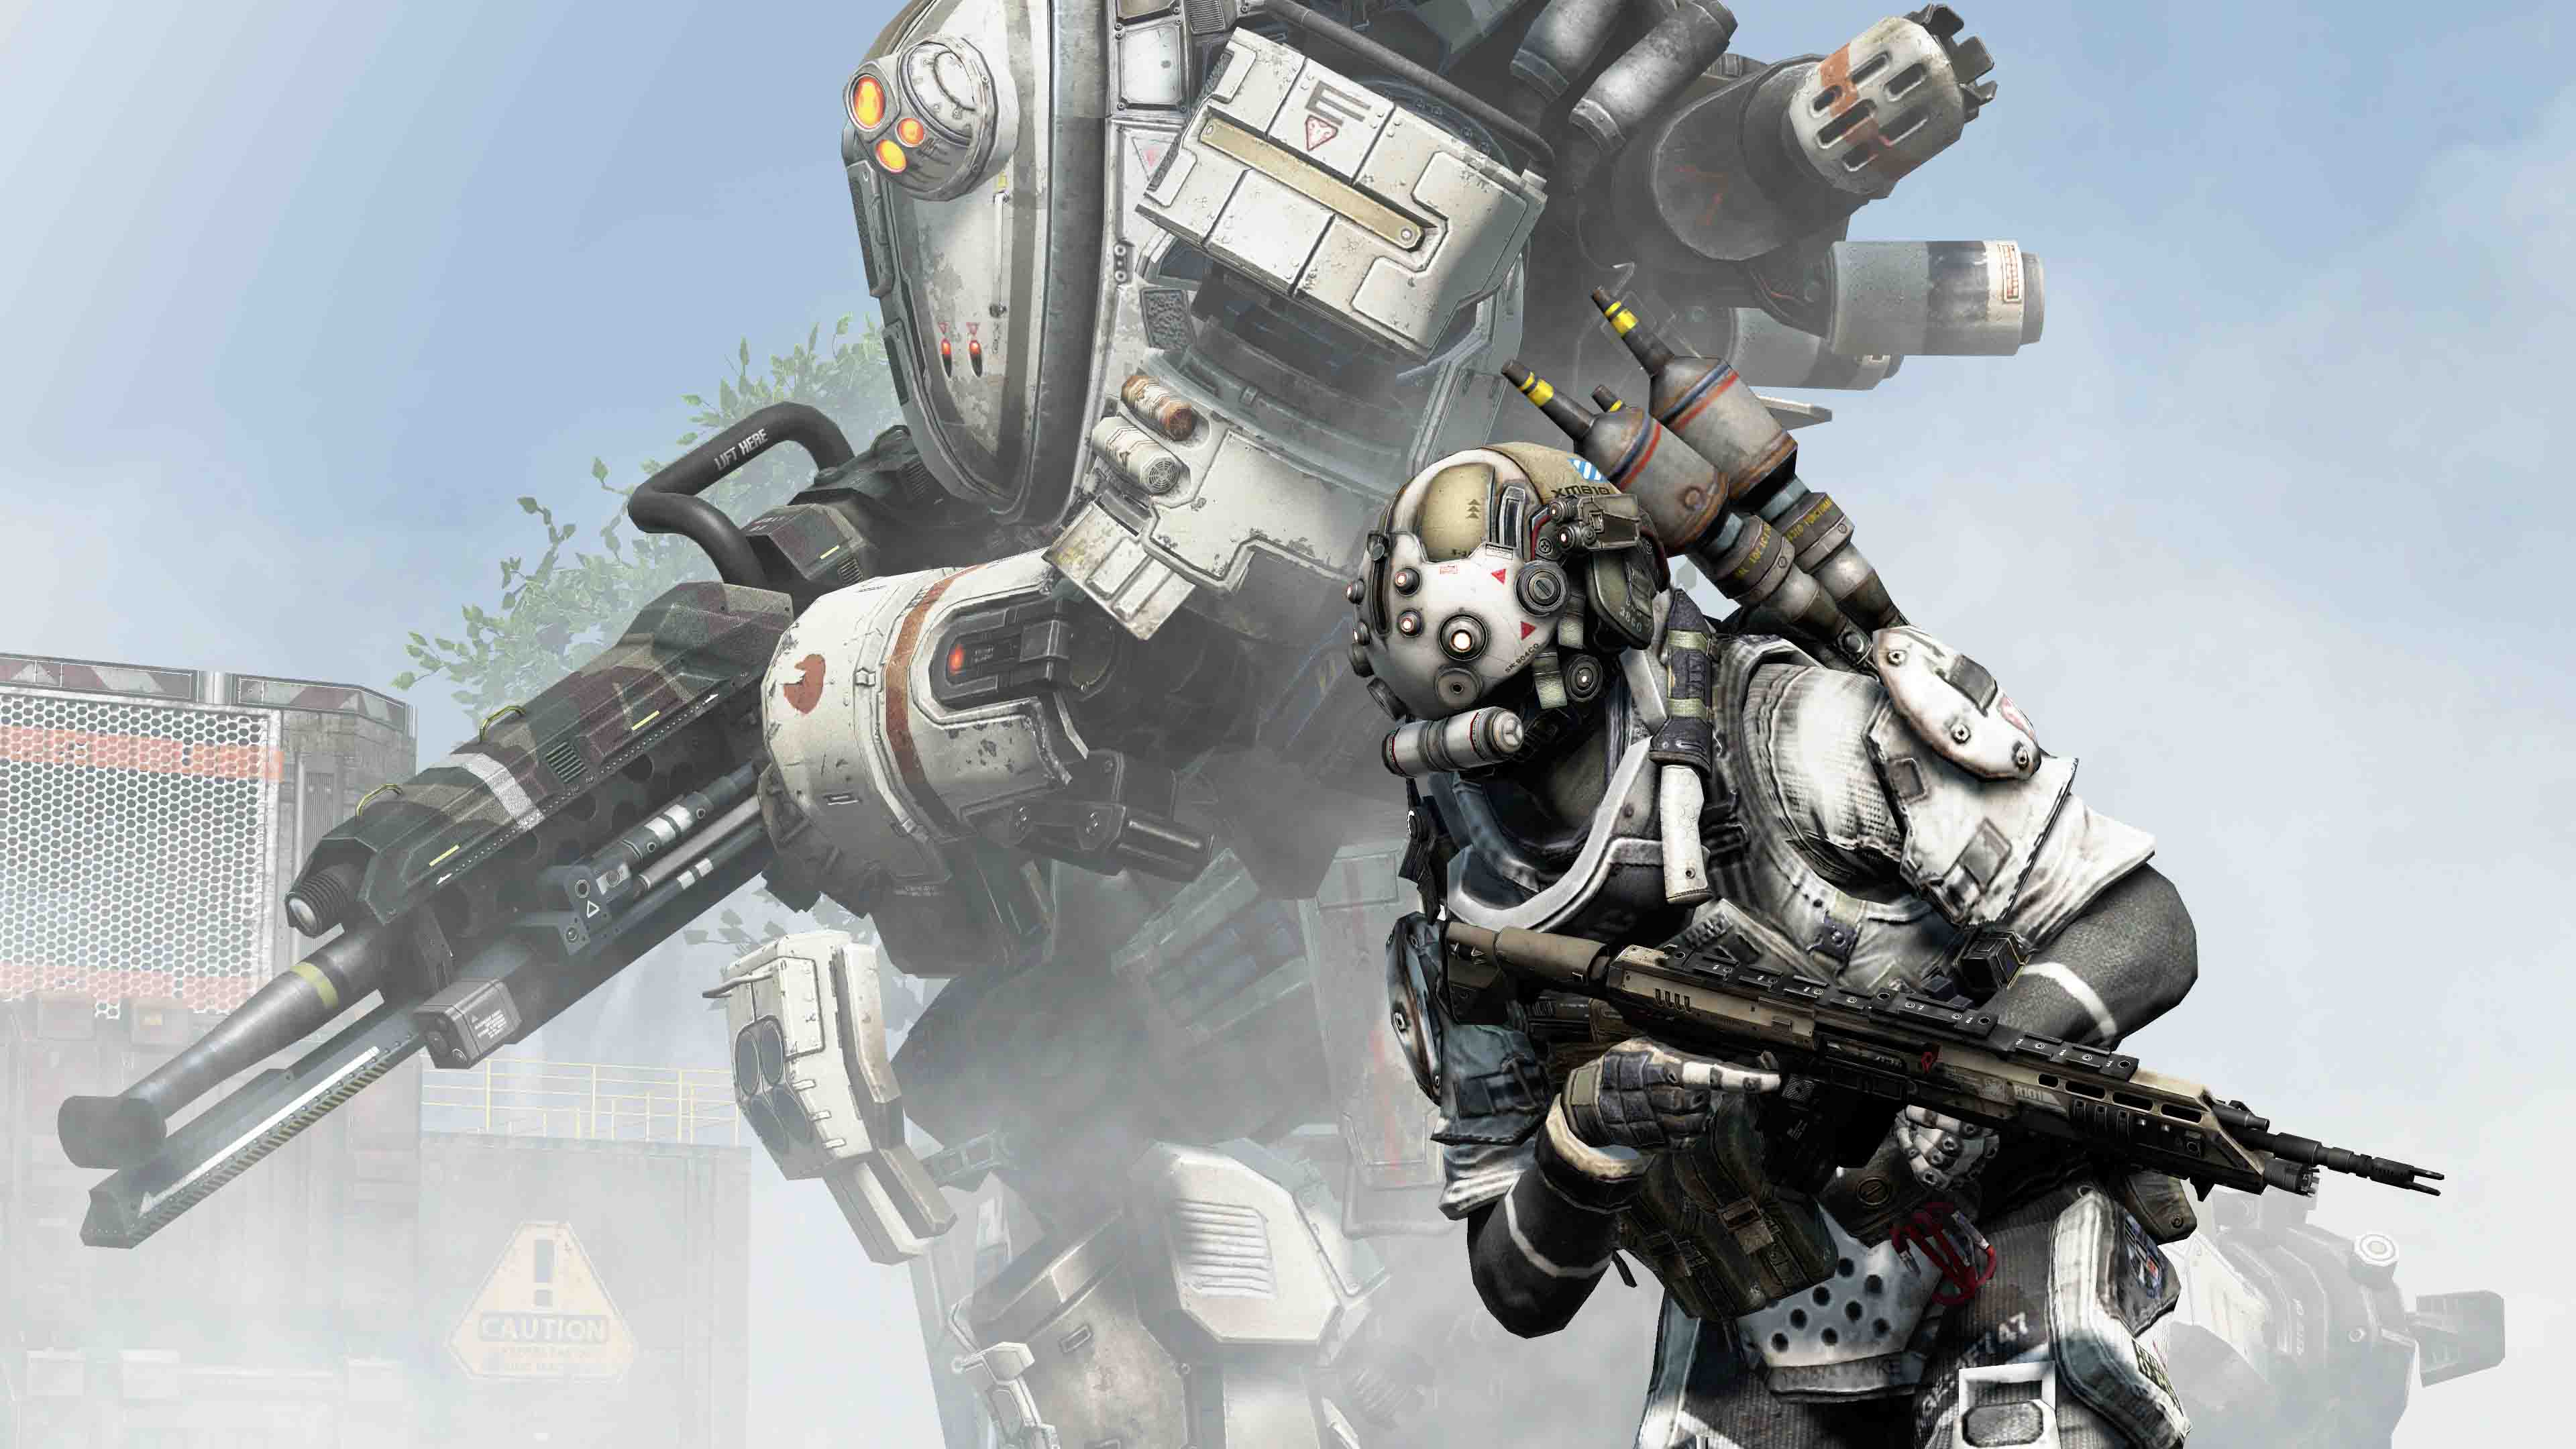
\includegraphics[keepaspectratio, height=\paperheight]{Titanfall.jpg}%
}}


\begin{document}
\AddToShipoutPicture*{\BackgroundPic}

\thispagestyle{empty}
%\vspace*{2em}
{\noindent\centering\Huge\TF titanfall:\\{\huge Genesys}\\[1em]{\Large\sffamily\bfseries A Titanfall Mod for the Genesys RPG\\v0.7.2}\\}
\vspace*{\fill}

\clearpage
\pagenumbering{roman}
\begin{multicols}{2}
\tableofcontents
\end{multicols}



\clearpage
\pagenumbering{arabic}
\setcounter{page}{1}


%%%%%
%Intro
%%%%%

\chapter{Welcome to the Militia}
\label{chap:intro}

Humanity lives in the deepest reaches of explored space in a vast region known as The Frontier. It contains many well-known and inhabited solar systems, but many more worlds remain uncharted. Most people will never travel this far away from normal civilization, but for pioneers, explorers, mercenaries, outlaws, and soldiers---the Frontier offers both adventure and opportunity.

The Interstellar Manufacturing Corporation (IMC) originally funded many expeditions to the Frontier, promising veterans of their military campaigns in the ``Core Systems"---the region of space containing the IMC's inhabited worlds including Earth---free land and other benefits in return for starting up businesses and colonies on the Frontier. Eventually, the IMC withdrew this support, leaving the colonists stranded without outside assistance for several decades.

Over time, life continued on the Frontier largely independent from the Core Systems. However, when the IMC returned several decades later to claim eminent domain over the Frontier's land, people and resources, the people of the Frontier united as the Frontier Militia, utilizing guerrilla and terrorist actions to further their cause.

This is where you come in. You grew up in the Frontier, it is your home. Now the IMC is back and claiming everything you worked your entire life for is theirs. It isn't. You know that, and now they need to learn it. Welcome to the Frontier Militia!


%%%%%
% Main Content
%%%%%

% New Character Options
% ---Archetypes
% ---Careers
% ---Heroic Abilities?
% Skills/Special Rules
% Talents
% Equipment
% ---Weapons
% ---Armour
% ---Gear
% Attachments
% ---Weapon attachments
% ---Armour attachments
% ---Titan attachments
% Vehicles
% ---Titans
% ---Other vehicles
% Adversaries



\chapter{Equipment}
\label{chap:equip}


\section{Sidearms}
\label{sec:sidearms}

\subsection{b3 Wingman}

\begin{wrapfigure}[4]{l}{.34\linewidth}
\vspace*{-2em}
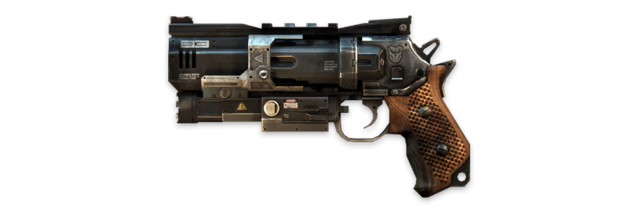
\includegraphics[width=\linewidth]{B3wingman}
\end{wrapfigure}

The B3 Wingman is an extremely powerful revolver with very high accuracy out to long ranges. Precision aim is required to mitigate the disadvantages of its very low rate of fire. 

\subsection{Hammond P2011}

\begin{wrapfigure}[4]{r}{.34\linewidth}
\vspace*{-2em}
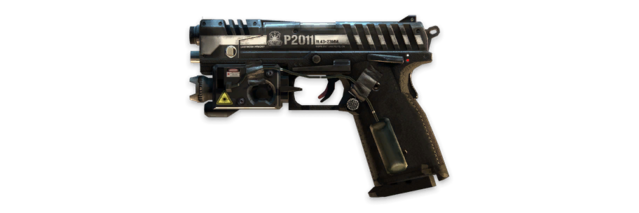
\includegraphics[width=\linewidth]{HammondP2011}
\end{wrapfigure}

The Hammond P2011 is a semi-automatic handgun with good accuracy and damage at range. Its integrated 'match trigger' allows it to be fired very rapidly, which is useful in close quarters. 

\subsection{RE-45 Autopistol}

\begin{wrapfigure}[3]{l}{.34\linewidth}
\vspace*{-2em}
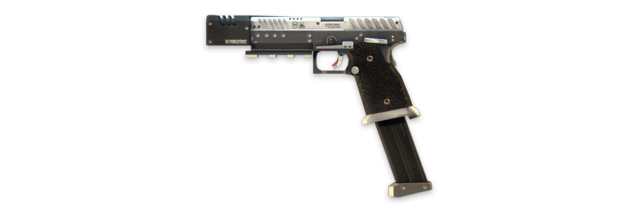
\includegraphics[width=\linewidth]{RE45Autopistol}
\end{wrapfigure}


The RE-45 is a fully automatic .45 caliber pistol, sacrificing damage and accuracy at longer distances for improved effectiveness at close range.

\subsection{Smart Pistol mkv}

\begin{wrapfigure}[7]{r}{.34\linewidth}
\vspace*{-2em}
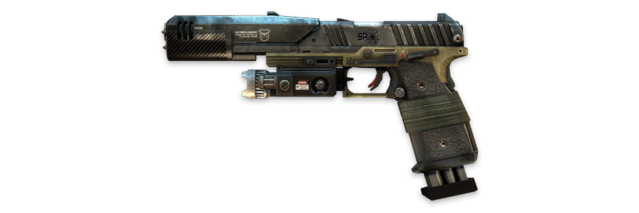
\includegraphics[width=\linewidth]{SmartPistolMK5}
\end{wrapfigure}

The Smart Pistol scans for hostile targets within a short range, locking onto them automatically. Any rounds fired will then maneuver to hit the locked targets. Aiming with the iron sights allows the operator to use the pistol in manual targeting mode. Due to the low magazine capacity, however, this weapon can run out of ammo by spending \Threat\Threat\Threat\ (instead of the normal \Despair). Spare ammunition for the smart pistol is twice the price as normal ammo, 50 credits.

\begin{table}[h!]
\caption{Sidearms}
\footnotesize
\begin{GenesysTable}{*{2}{l} *{2}{c} l c c r c X[l]}
Name & Skill & Dam & Crit & Range & Enc & HP & Price & Rarity & Special\\
B3 Wingman & Ranged (Light) & 6 & 3 & Medium & 1 & 1 & 500 & 3 & \\
Hammond P2011 & Ranged (Light) & 5 & 4 & Medium & 1 & 1 & 150 & 3 & \\
RE-45 Autopistol & Ranged (Light) & 5 & 3 & Short & 2 & 1& 300 & 6 & Accurate 1 \\
Smart pistol mk5 & Ranged (Light) & 5 &  3 & Short & 1 & 1 & 450 & 8 & Guided 3, Special\\

\end{GenesysTable}
\end{table}


\pagebreak
\section{Longarms}
\label{sec:rifles}

\subsection{R101C Carbine}
\begin{wrapfigure}[2]{l}{.34\linewidth}
\vspace*{-2em}
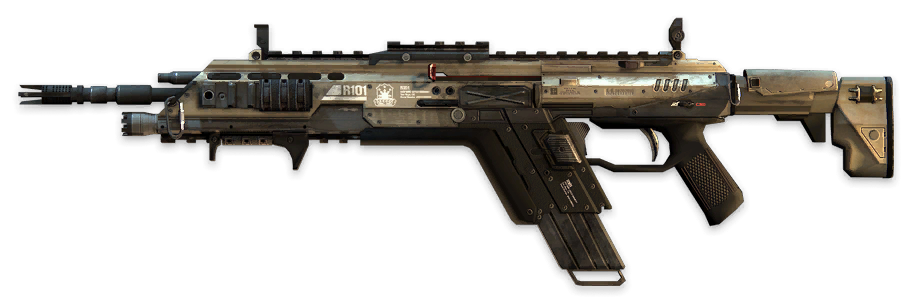
\includegraphics[width=\linewidth]{R101CCarbine}
\end{wrapfigure}


The R-101C is a fully automatic, compact assault weapon commonly used throughout the Frontier. 


\subsection{Hemlock BF-R}
\begin{wrapfigure}[5]{r}{.36\linewidth}
\vspace*{-2em}
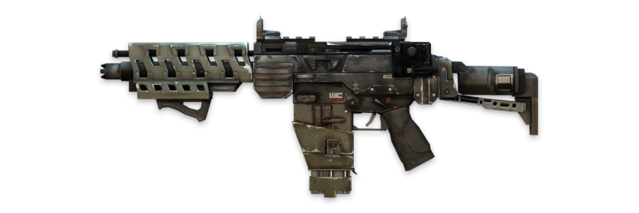
\includegraphics[width=\linewidth]{HemlokBFR}
\end{wrapfigure}
The factory issue Hemlok fires a three-round burst. While this can be a liability at short range, this tradeoff allowed the engineers at TW Ordnance to deliver a weapon with a good balance of long-range accuracy, damage, and fire rate.

\subsection{G2A4 Battle Rifle}
\begin{wrapfigure}[4]{l}{.36\linewidth}
\vspace*{-2em}
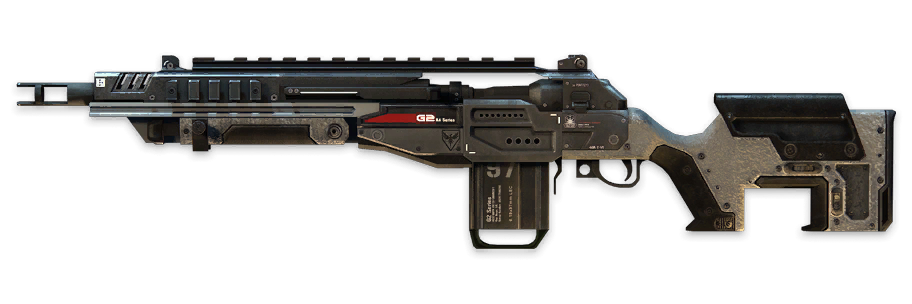
\includegraphics[width=\linewidth]{G2A4Rifle}
\end{wrapfigure}


Despite recent advances in weapons technology, the older G2A4 semi-automatic rifle remains a favorite of special forces units due to its high damage and extremely precise fire---a testament to its high level of craftsmanship.

\subsection{EVA-8 Shotgun}
\begin{wrapfigure}[5]{r}{.36\linewidth}
\vspace*{-2em}
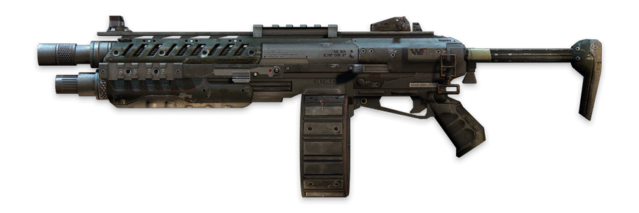
\includegraphics[width=\linewidth]{EVA8Shotgun}
\end{wrapfigure}


The EVA-8 is a semi-automatic shotgun, originally designed for extra-vehicular activity, both in conventional and in exo-atmospheric conditions. The low capacity and quick trigger means that the EVA-8 can run out of ammo by spending \Threat\Threat\Threat\ (instead of the normal \Despair).

\subsection{R-97 Compact SMG}
\begin{wrapfigure}[3]{l}{.36\linewidth}
\vspace*{-2em}
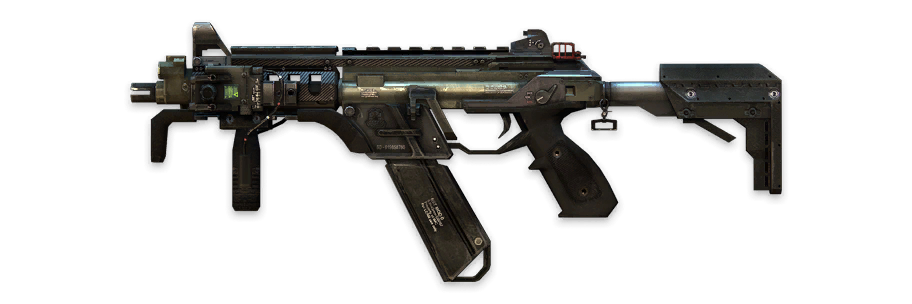
\includegraphics[width=\linewidth]{R97CompactSMG}
\end{wrapfigure}

The R-97 is a compact submachine gun that excels at close-quarters combat, due to its extremely high rate of fire and minimal recoil.

\subsection{C.A.R. SMG}
\begin{wrapfigure}[4]{r}{.36\linewidth}
\vspace*{-2em}
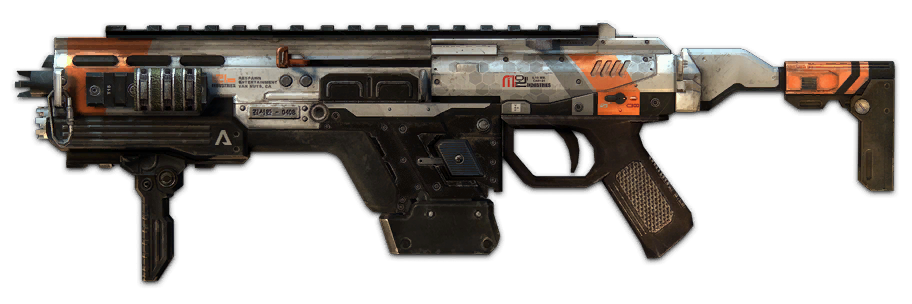
\includegraphics[width=\linewidth]{CARSMG}
\end{wrapfigure}

The C.A.R. (Combat Advanced Round) submachine gun is designed to fire a more powerful round that provides greater damage and accuracy at range, at the cost of fire rate and capacity.


\subsection{D-101 Longbow DMR}
\begin{wrapfigure}[3]{l}{.36\linewidth}
\vspace*{-2em}
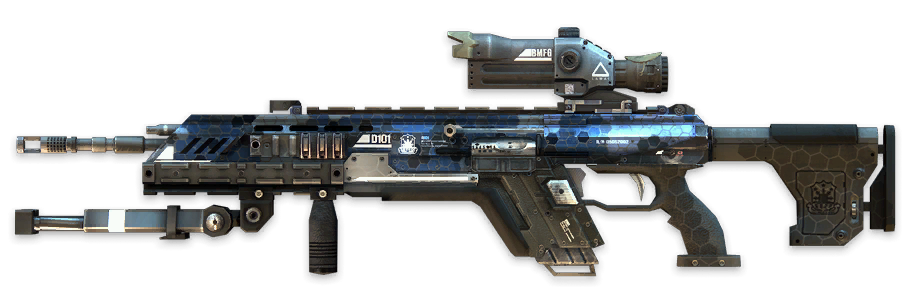
\includegraphics[width=\linewidth]{LongbowDMRSniper}
\end{wrapfigure}

The Longbow-DMR is a semi-automatic sniper rifle. Its hyper-velocity round completely eliminates the need to lead targets, and allows the shooter to fire multiple shots quickly in succession.


\subsection{Kraber-AP Sniper}
\begin{wrapfigure}[4]{r}{.36\linewidth}
\vspace*{-2em}
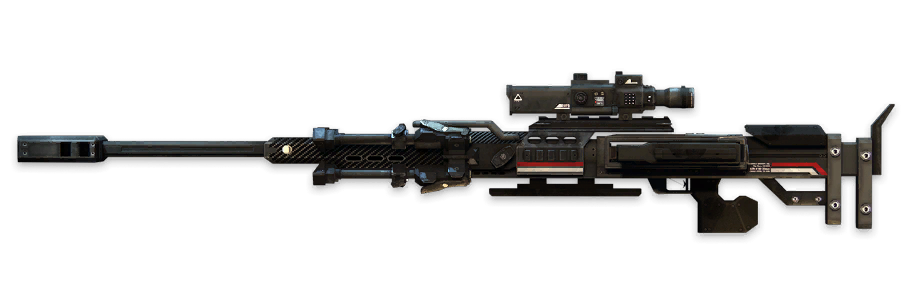
\includegraphics[width=\linewidth]{KraberAPSniper}
\end{wrapfigure}

The Kraber fires a unique round that ensures 'one-shot, one-kill' results against human-scale targets. However, considerable judgement in leading is required, making this a difficult weapon to use against moving targets.

\subsection{Spitfire LMG}
\begin{wrapfigure}[4]{l}{.36\linewidth}
\vspace*{-2em}
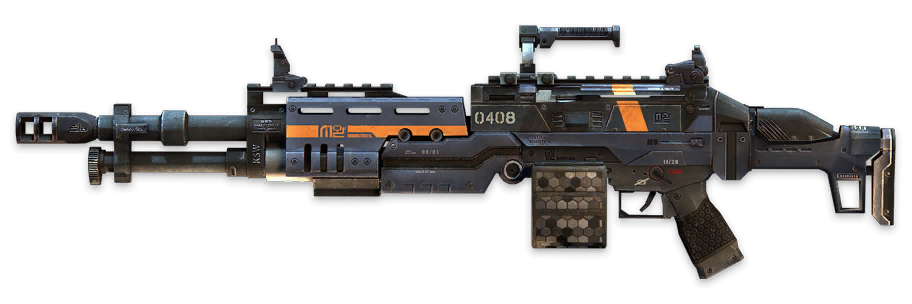
\includegraphics[width=\linewidth]{SpitfireLMG}
\end{wrapfigure}

The Spitfire Light Machine Gun recoils heavily when first fired, but quickly settles into a tight firing pattern. The manufacturer strongly recommends sustained saturating fire, instead of short controlled bursts.


\begin{table}[h!]
\caption{Longarms}
\footnotesize
\begin{GenesysTable}{*{2}{l} *{2}{c} l c c r c X[l]}
Name & Skill & Dam & Crit & Range & Enc & HP & Price & Rarity & Special\\
R-101C Carbine & Ranged (Heavy) & 8 & 3 & Long & 4 & 2 & 1,050 & 7 & Auto-fire\\
Hemlock BF-R & Ranged (Heavy) & 8 & 3 & Long & 4 & 2 & 1,000 & 7 & Accurate 1\\
G2A4 Battle Rifle & Ranged (Heavy) & 8 & 3 & Long & 4 & 2 & 950 & 6 &  \\ 
EV-8 Shotgun & Ranged (Heavy) & 8 & 3 & Short & 3 & 2 & 625 & 4 & \Special{Blast 6, Knockdown, Special}
R-97 SMG & Ranged (Heavy) & 6 & 3 & Medium & 3 & 2 & 750 & 6 & \Special{Auto-fire, Accurate 1}
C.A.R. SMG & Ranged (Heavy) & 7 & 3 & Medium & 3 & 2 & 550 & 6 & \Special{Accurate 2, Limited Ammo 2}
Longbow DMR & Ranged (Heavy) & 9 & 3 & Long & 4 & 2 & 1,000 & 5 & Accurate 1\\
Kraber & Ranged (Heavy) & 12 & 2 & Extreme & 5 & 3 & 2,000 & 8 & \Special{Accurate 2, Limited Ammo 1, Pierce 2}
Spitfire LMG & Gunnery &10 & 3 & Long & 6 & 3 & 1,750 & 6 & \Special{Auto-fire, Cumbersome 2, Pierce 2, Vicious 2}
\end{GenesysTable}
\end{table}

\section{Pilot Ordnance}
\label{sec:pilotordnance}

\subsection{Special Rules}
\textbf{Set Explosives.} The arc mine is an unusual ordnance in that you don't throw it at your opponent but rather set it in place and wait for someone to trigger the explosion. As an action you may set up to two mines within Engaged range of you. Then, when someone or something enters engaged range with the mine you make an Engineering combat check against the target.


\subsection{Arc Grenade}
\begin{wrapfigure}[4]{r}{.36\linewidth}
\vspace*{-2em}

\includegraphics[width=\linewidth]{ArcGrenade}
\end{wrapfigure}

The Arc Grenade is by infantry of the IMC and Militia. When activated, the Arc Grenade explodes in a blast of Arc energy capable of short circuiting and dealing heavy damage to robotic units and equipment such as Titans, Spectres, Stalkers, HUDs and optical equipment found within the helmet of a Pilot and Reapers. An arc grenade can negate Defense granted by energy shields by spending \Advantage\Advantage.

\subsection{Arc Mine}
\begin{wrapfigure}[6]{l}{.36\linewidth}
\vspace*{-2em}\centering
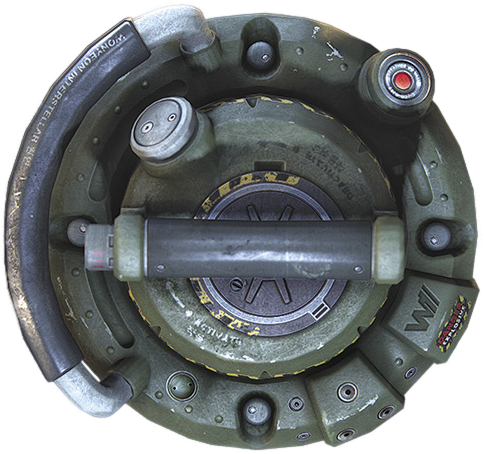
\includegraphics[width=0.5\linewidth]{ArcMine}
\end{wrapfigure}

The Arc Mine is a proximity mine that can stick on any surface. It takes 1 second after sticking to something to arm. Arc Mines won't explode until an enemy Pilot, Titan, Grunt, or Spectre enter the mine's range. An arc mine can negate Defense granted by energy shields by spending \Advantage\Advantage.

\subsection{Electric Smoke Grenade}
A pilot-portable version of the Titan defense system, this ``grenade" is designed to obscure an area and disperse pilots in an entrenched position. Any non-Titan target who stays within the cloud must make a \textbf{Hard (\DifficultyDie\DifficultyDie\DifficultyDie) Resilience check} at the end of their next turn or suffer 3 strain, plus 1 additional strain per \Failure. If the check generates \Threat\Threat, you may activate the Disorient quality.

The cloud creates two dice worth of concealment and completely blocks the Guided weapon quality on any attack against a target within the cloud or if the weapon must target through the cloud.

\subsection{Firestar}
The firestar is an incendiary throwing star that creates thermite on impact. It will stick to surfaces and enemies alike.


\subsection{Frag Grenade}
\begin{wrapfigure}[2]{r}{.36\linewidth}
\vspace*{-2em}

\includegraphics[width=\linewidth]{FragGrenade}
\end{wrapfigure}

The basic explosive device known to all modern soldiers, the Frag Grenade is still an incredibly useful weapon.

\subsection{Satchel Charge}
\begin{wrapfigure}[6]{l}{.36\linewidth}
\vspace*{-2em}
\centering
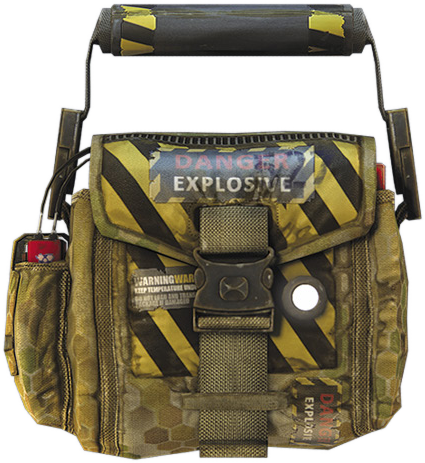
\includegraphics[width=.4\linewidth]{SatchelCharge}
\end{wrapfigure}

Satchel Charges stick to any surface and are manually detonated, causing massive explosive damage to anything nearby. Like mines, satchel charges are set and triggered to explode. Unlike a mine, however, you must trigger them yourself. As an action you may place up to two charges within Engaged range. As an out-of-turn incidental you may detonate the charges, making an Engineering combat check against the target.


\begin{table}[h!]
\caption{Ordnance}
\footnotesize
\begin{GenesysTable}{*{2}{l} *{2}{c} l c c r c X[l]}
Name & Skill & Dam & Crit & Range & Enc & HP & Price & Rarity & Special\\
Arc Grenade & Ranged (Light) & 5 & 4 & Short & 1 & 0 & 55 & 6 & \Special{Blast 4, Disorient 2, Limited Ammo 1, Stun Damage, Special}
Arc Mine & Mechanics & 6 & 4 & Engaged & 3 & 0 & 70 & 7 & \Special{Blast 5, Disorient 2, Limited Ammo 1, Stun Damage, Special}
Electric Smoke & Ranged (Light) & 4 & 6 & Short & 1 & 0 & 50 & 7 & \Special{Blast 3, Disorient 2, Limited Ammo 1, Stun Damage, Special}
Firestar & Ranged (Light) & 8 & 2 & Short & 1 & 0 & 100 & 7 & Burn 1, Limited Ammo 1\\
Frag Grenade & Ranged (Light) & 8 & 3 & Short & 1 & 0 & 90 & 7 & \Special{Blast 6, Limited Ammo 1}
Satchel Charge & Mechanics & 12 & 2 & Engaged & 2 & 0 & 280 & 6 & \Special{Blast 8, Breach 1, Limited Ammo 1, Special}
\end{GenesysTable}
\end{table}



\section{Anti-Titan Weapons}
\label{sec:antititanweapons}


\subsection{Archer Heavy Rocket}
\begin{wrapfigure}[4]{r}{.36\linewidth}
\vspace*{-2em}
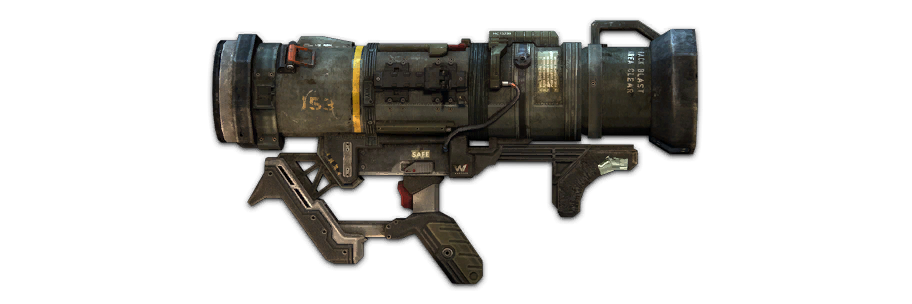
\includegraphics[width=\linewidth]{ArcherHeavyRocket}
\end{wrapfigure}

The Archer fires a powerful homing rocket. It must be locked onto a target before it can be fired. When aimed, a targeting window flips out, allowing target acquisition. Hold this window over the target continuously until a lock is achieved, then fire. The Guided quality can only be activated when attacking targets made of significant metal content, like Titans and Spectres. Reload rockets for the Archer cost 3,000 credit.

\subsection{Charge Rifle}
\begin{wrapfigure}[4]{l}{.36\linewidth}
\vspace*{-2em}
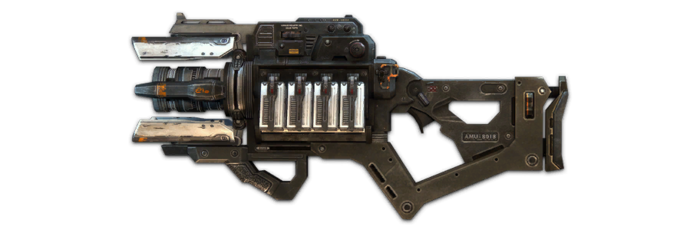
\includegraphics[width=\linewidth]{ChargeRifle}
\end{wrapfigure}

The Charge Rifle fires an energy beam that inflicts massive damage. Holding the trigger charges the weapon. Timing is critical to its use: this weapon will only fire when it reaches full charge, and it will discharge automatically as soon as it hits full charge.



\subsection{Mag Launcher}
\begin{wrapfigure}[3]{r}{.36\linewidth}
\vspace*{-2em}
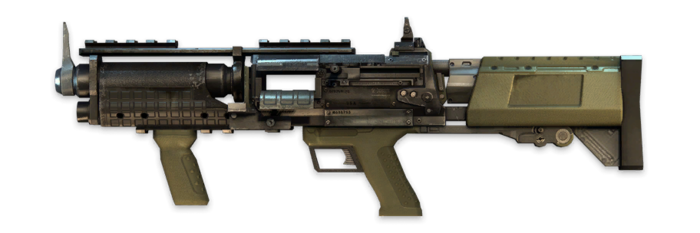
\includegraphics[width=\linewidth]{MagLauncher}
\end{wrapfigure}


The Mag Launcher fires magnetic grenades. When fired, the grenades will veer towards nearby enemy Titans and Spectres, and detonate on impact. The Guided quality can only be activated when attacking targets made of significant metal content, like Titans and Spectres. Due to the low magazine capacity, however, this weapon can run out of ammo by spending \Threat\Threat\Threat\ (instead of the normal \Despair).

\subsection{Sidewinder}
\begin{wrapfigure}[5]{l}{.36\linewidth}
\vspace*{-2em}
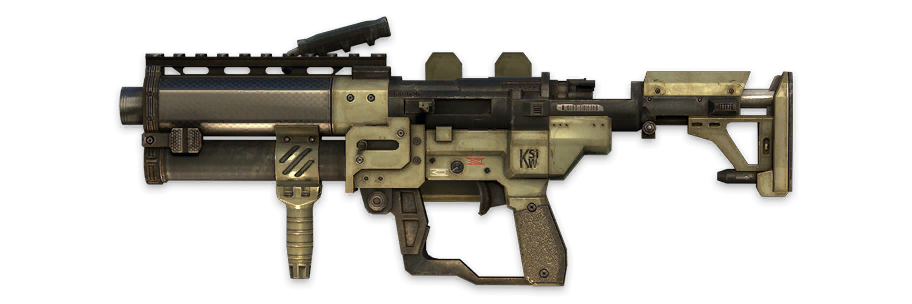
\includegraphics[width=\linewidth]{Sidewinder}
\end{wrapfigure}

The Sidewinder is a rapid-fire micro-missile launcher. It is effective against large targets, but lacks precision due to its large spread. The micro-missiles it fires do not yield a large area effect on detonation, due to their shaped-charge design.


\begin{table}[h!]
\caption{Anti-Titan Weapons}
\footnotesize
\begin{GenesysTable}{*{2}{l} *{2}{c} l c c r c X[l]}
Name & Skill & Dam & Crit & Range & Enc & HP & Price & Rarity & Special\\
Archer Rocket & Gunnery & 30 & 2 & Extreme & 8 & 4 & 10,525 & 8 & \Special{Blast 20, Breach 2, Cumbersome 3, Guided 3, Limited Ammo 1, Prepare 1}
Charge Rifle & Gunnery & 9 & 2 & Extreme & 8 & 4 & 3,250 & 7 & \Special{Accurate 1, Breach 2, Cumbersome 2, Slow-Firing 1, Vicious 2}
Mag Launcher & Gunnery & 12 & 3 & Long & 6 & 3 & 3,450 & 7 & \Special{Breach 2, Guided 2, Special}
Sidewinder & Gunnery & 18 & 2 & Medium & 6 & 3 & 5,075 & 6 & \Special{Auto-fire, Breach 2, Cumbersome 2, Inaccurate 1, Limited Ammo 3, Vicious 1}
\end{GenesysTable}
\end{table}

\section{Armour}

\subsection{Armoured Carapace}
Armoured carapace completely covers the wearer from head to toe and with the right attachments can be environmentally sealed. The carapace has a rigid outer shell that deflects or blocks incoming attacks. It is also designed to be extremely customizable, with one more hard point than a comparable size armour would otherwise have.


\subsection{Flak Vest}
Made from lightweight polymers and ballistic fabrics, this armour provides decent protection against small arms fire and shrapnel.

\subsection{Heavy Jacket}

Not a form of combat armour, but a well-made jacket does provide limited protection.


\begin{table}[h!]
\centering
\caption{Armour}
\footnotesize
\begin{GenesysTable}{l *{4}{c} r c}
Type & Defense & Soak & Enc. & HP & Price & Rarity\\
Armoured Carapace & 1 & +2 & 4 & 3 & 850 & 6\\
Flak Vest & 0 & +2 & 3 & 2 & 500 & 5\\
Heavy Jacket & 0 & +1 & 1 & 1 & 50 & 1\\
\end{GenesysTable}
\end{table}

\section{Gear}

A Militia Titan pilot needs more than just a good weapon and heavy armour to defeat the IMC and drive them from their home. In this section you'll find the more mundane---but no less important---items that makes a Militia pilot more than a grunt with a gun.

\subsection{Comm-Bead}
This communications device fits into a sentient?s ear (or other auditory orifice) and allows them to communicate with friends and allies within 100 kilometers. If the comm-bead can tie into a planetary communications network (the kind that any civilized planet has), then it can communicate with anyone on the same planet.

An encrypted version of the comm-bead is also available. Any attempt to hack into the encrypted communication is upgraded twice.

\subsection{Cybernetics}
See \emph{Genesys} Core Rulebook page 177.


\subsection{Data Knife}
The Data Knife is a tool used to hack into enemy Spectres, turrets or other computing devices. It has an on-board AI programmed specifically to hack into enemy computers. It has 2 ranks in the Hacking skill. If left to its own devices it will roll \AbilityDie\AbilityDie\ for hacking checks. If you spend your action hacking, it instead assists you in your attempt (see pages 26--27 of the \emph{Genesys} Core Rulebook).


\subsection{First Aid Kit}
A first aid kit has all the basics you need to tend to minor battlefield injuries. This kit provides your character with the equipment needed to make Medicine checks to heal wounds or Critical Injuries without penalty. However, \Threat\Threat\Threat\ or \Despair\ means your character has used all of the kit?s supplies.

\subsection{Jump Kit}
Jump Kits provide a brief burst of thrust that is used to leap to higher locations. They also have a function that adjusts the deceleration on potentially fatal descents to safe levels, allowing Pilots to fall from great heights without injury.

When armed with a jump kit, upgrade all Athletics checks to climb and jump and ignore difficult terrain as long as you can bypass it via a nearby wall or other outcropping. In addition, reduce the overall distance fallen by one range band.

\subsection{Night Optics}
These goggles allows the wearer to see in the dark. When wearing night optics, your character
removes up to \SetbackDie\SetbackDie\ added to their checks due to darkness.


\subsection{Pain Killers}
See page 94 of the \emph{Genesys} Core Rulebook.


\subsection{Portable Medkit}
A well-equipped portable medkit comes with every- thing someone might need to treat all manner of injuries, from bullet wounds to broken legs.

A portable medkit allows your character to perform Medicine checks to heal wounds and Critical Injuries without penalty. The inclusion of modern drugs adds automatic \Advantage\ to the check results.

\subsection{Pulse Blade}
the pulse blade can be thrown and also provides a brief sonar pulse that can detect enemies even through walls.

As an action, a character may make an \textbf{Average (\DifficultyDie\DifficultyDie) Ranged (Light) check} to secure the blade to any solid surface within short range, including the hull of a Titan. On a success it sends out a sonar pulse that reveals the current location of all enemies within short range. At the beginning of the next round another sonar pulse is released. Any cloaked target looses the benefit of the cloak until the leave the area of effect.

The pulse blade can also be used as a weapon with the following profile: Ranged (Light); damage +1; crit 4; Range (Short); Limited Ammo 1, Pierce 1.

\begin{table}[h!]
\centering
\caption{Gear}
\footnotesize
\begin{GenesysTable}{l c r c}
Item & Enc & Price & Rarity\\
Comm-Bead & 0 & 25 & 1\\
Comm-Bead, encrypted & 0 & 2,000 & 5\\
Data Knife & 0 & 500 & 5\\
First Aid Kit & 1 & 100 & 3\\
Jump Kit & 2 & 1,000 & 7\\
Night Optics & 0 & 500 & 5\\
Painkillers & 0 &25 & 2\\
Portable Medkit & 2 & 200 & 4\\
Pulse Blade & 1 & 150 & 5\\
\end{GenesysTable}
\end{table}

\chapter{Item Attachments}
Item attachments follow the rules on pages 206--209 of the \emph{Genesys} Core Rulebook. Many of the attachments in that section are available in \emph{Titanfall: Genesys} as well as new attachments described below.

\section{Weapon Attachments}

The following weapon attachments are available to characters in the \emph{Titanfall: Genesys} setting. In addition, several attachments from the \emph{Genesys} Core Rulebook are available.

Italicized attachments are new and found in the following section.


\begin{table}[h!]
\centering
\caption{Weapon Attachments}
\footnotesize
\begin{GenesysTable}{l c r c}
Attachment & HP required & Price & Rarity\\
Bipod Mount & 1 & 250 & 2\\
\emph{Dataspike} & 1 & 500 & 6\\
\emph{Enhanced Targeting Algorithm} & 1 & 800 & 7\\
Extended barrel & 2 & 1,000 & 4\\
Hair Trigger & 1 & 150 & 3\\
\emph{Holosight} & 1 & 500 & 4 \\
\emph{Laser Sight} & 1 & 500 & 5\\
\emph{Silencer} & 1 & 100 & 5\\
Superior Customization & 1 & 750 & 7\\
Telescopic Sight & 1 & 200 & 3\\
Tripod Mount & 2 & 400 & 3\\
Under-barrel Weapon & 2 & Varies & Varies\\
Weapon sling & 1 & 250 & 1\\
\end{GenesysTable}
\end{table}


\subsection{Dataspike}
The Dataspike is a tool used to hack into enemy Spectres, turrets or other computing devices. It has an on-board AI programmed specifically to hack into enemy computers. \\
\noindent\textbf{Use With:} The dataspike is specifically designed to be used with the combat knife.\\
\noindent\textbf{Modifiers:} Dataspikes can perform Hacking checks for a player with a Hacking skill of 2 and an Intellect of 0. If unassisted it rolls \AbilityDie\AbilityDie\ for Hacking checks (see pages 26--27 of the \emph{Genesys} Core Rulebook for rules on assisted checks).\\
\noindent\textbf{Hard Points Required:} 1\\
\noindent\textbf{Price:} 500

\subsection{Enhanced Targeting Algorithm}
While most guided weaponry is good as-is, many users tweak the targeting code to acquire a lock faster.\\
\noindent\textbf{Use With:} Any weapon with the Guided quality may have this attachment.\\
\noindent\textbf{Modifiers:} When you preform the aim manoeuvre you may add \Advantage\ instead of \BoostDie\ to your combat check.\\
\noindent\textbf{Hard Points Required:} 1\\
\noindent\textbf{Price:} 800


\subsection{Holosight}
This device projects a hologram of a crosshair a meter or so in front of the barrel to aid in aiming the weapon. Unfortunately that also makes it easier to spot the shooter.\\
\noindent\textbf{Use With:} Any firearm can have a holosight added.\\
\noindent\textbf{Modifiers:} The shooter may aim as an incidental once per round at a target up to medium range. If the holosight is used, reduce any concealment dice the shooter is benefiting from by 1 until the beginning of the character's next turn (see page 110 of the \emph{Genesys} Core Rulebook for concealment rules).\\
\noindent\textbf{Hard Points Required:} 1\\
\noindent\textbf{Price:} 500

\subsection{Laser Sight}
A simple and lower-tech solution than most on the Frontier are used to, it is a classic for a reason. A laser sight emits a low-level light beam that places a physical dot where the weapon is pointing. But due to the low output it has limited range.\\
\noindent\textbf{Use With:} Any firearm can have a laser sight attached.\\
\noindent\textbf{Modifiers:} A laser sight adds the Accurate 1 quality, or increases an existing Accurate quality by 1.\\
\noindent\textbf{Hard Points Required:}  1\\
\noindent\textbf{Price:} 500

\subsection{Silencer}
A silencer makes it harder for others to pinpoint the location of shots made with the weapon it is attached to.\\
\noindent\textbf{Use With:} Any firearm can have a silencer attached.\\
\noindent\textbf{Modifiers:} Adds \SetbackDie\SetbackDie\ to any Perception or Vigilance checks to locate the shooter firing the weapon.\\
\noindent\textbf{Hard Points Required:}  1\\
\noindent\textbf{Price:} 100


\section{Armour Attachments}

The following armour attachments are available to characters in the \emph{Titanfall: Genesys} setting. In addition, several attachments from the \emph{Genesys} Core Rulebook are available.

Italicized attachments are new and found in the following section.

\begin{table}[h!]
\centering
\caption{Armour Attachments}
\footnotesize
\begin{GenesysTable}{l c r c}
Attachment & HP required & Price & Rarity\\
Deflective Plating & 1 & 450 & 4\\
Enhanced Lifting Servos & 2 & 1,500 & 5\\
\emph{Extra Emitters} & 1 & 2,000 & 6\\
\emph{Extra Padding} & 1 & 300 & 6\\
\emph{Grapple Launcher} & 2 & 350 & 3\\
Reinforced Plating & 2 & 8,000 & 7\\
\emph{Stim Injectors} & 1 & 2,500 & 5\\
Vacuum Sealed & 1 & 600 & 4\\
\end{GenesysTable}
\end{table}





\subsection{Grapple Launcher}
The grapple launcher has a weighted head designed to pierce and hold firm to any solid surface. It allows the wearer to traverse longer distances than normal---even straight up! Whether you're trying to get away, close the distance or get in or out of a secure site in a hurry, the grapple launcher is just what you need. Some crazy pilots even use it to rodeo a Titan!\\
\noindent\textbf{Use With:} This attachment can be applied to any armor.\\
\noindent\textbf{Modifiers:} As an action, a character may make an \textbf{Average (\DifficultyDie\DifficultyDie) Ranged (Light) check} to secure the grapple launcher on any solid object within short range. On a success, they may, as a manoeuvre, reel in the cord and pull themselves towards the the object. If the object is unsecured, it instead is pulled to the character. \\
\noindent\textbf{Hard Points Required:} 2\\
\noindent\textbf{Price:} 350

\subsection{Extra Emitters}
Outfitting a cloaking device with extra emitters makes the cloak even more believable and provides even more protection to the soldier wearing it.\\
\noindent\textbf{Use With:} This attachment can be applied to the cloaking device.\\
\noindent\textbf{Modifiers:} Increase the cloaking device's Defense to 3.\\
\noindent\textbf{Hard Points Required:} 1\\
\noindent\textbf{Price:} 2,000

\subsection{Extra Padding}
This attachment adds a layer of padding to the cloaking device to help absorb the impact of weapons that are not fooled by the illusion.\\
\noindent\textbf{Use With:} This attachment can be applied to the cloaking device.\\
\noindent\textbf{Modifiers:} Increase the cloaking device's soak by +1.\\
\noindent\textbf{Hard Points Required:} 1\\
\noindent\textbf{Price:} 300


\subsection{Stim Injectors}
Stim injectors, or simply 'stims' to those who use them, are used for brief bursts of speed on the battlefield. On command they inject a potent cocktail of adrenaline and various pharmaceuticals that increase speed and reaction time. While it enables characters to get where they're going faster, it does stress the user's system.\\
\noindent\textbf{Use With:} This attachment can be applied to any armor.\\
\noindent\textbf{Modifiers:} Once per round on your turn after you have performed two manoeuvres you may suffer 1 strain to perform the move manoeuvre as an incidental. At the end of any encounter where your character used the stim injectors, they suffer 3 additional strain.\\
\noindent\textbf{Hard Points Required:} 1\\
\noindent\textbf{Price:} 2,500

\chapter{Titans}
\label{chap:titans}

Titans are mech-style robots, descended from modern-day fledgling military exoskeletons, designed for both civilian and military applications. 

There are three classes of titans, as described below.

\section{Special Rules}
\label{sec:specialrules}

All titans have the following special rule:

\textbf{Mecha Chassis:} As long as a Titan's propulsion isn't compromised it ignores the speed requirement for the reposition maneuver.

\section{Stryder}
\label{sec:stryder}
\begin{wrapfigure}[13]{r}{.34\linewidth}
\vspace*{-2em}
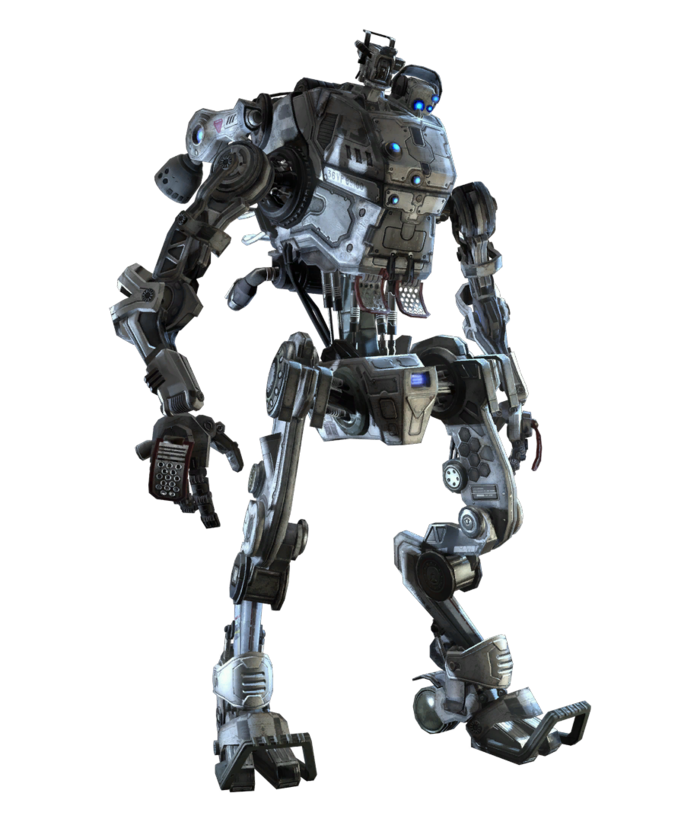
\includegraphics[width=\linewidth]{Stryder}
\end{wrapfigure}


The Stryder is a Titan chassis developed and manufactured by Hammond Robotics. Developed as an extremely mobile and maneuverable Titan variant, the Stryder's almost skeletal design has been optimized for superior speed and agility. Significant improvements have been made to its Dash Core, while the Titan can also sprint for greater distances, making it perfect for hit-and-run attacks, ambushes and rapid redeployments. Unfortunately, this speed comes at a price. The Stryder's design is stripped down compared to other Titan variants, and its armor is largely non-existent, making it much more fragile in combat. In Titan-vs-Titan engagements, Stryder Pilots must use all available cover and their machine's impressive speed to outflank and evade their heavier adversaries, as they are unlikely to survive a straight-up slug-fest.

\textbf{Dash Core}: The Stryder-class Titan has an in-built dash core. Once per round on your turn, you may cause the titan to suffer 1 system strain to perform the Evade maneuver as an Incidental, ignoring the Speed requirement.

\vspace{2em}

\Vehicle{3}{3}{+2}{2}{1}{13}{20}

\begin{multicols}{2}
\noindent\textbf{Control Skill:} Pilot (Titan)\\
\noindent\textbf{Complement:} One pilot\\
\noindent\textbf{Passenger Capacity:} None\\
\noindent\textbf{Price/Rarity:} 20,750/8\\
\noindent\textbf{Consumables:} None\\
\noindent\textbf{Encumbrance Capacity:} 2\\
\noindent\textbf{Weapons:} Titan punch (Pilot [Titan]; Damage 2; Critical 3; Range [Engaged]; Accurate 1)\\
\noindent\textbf{Hard Points:} 3
\end{multicols}

\section{Atlas}
\label{sec:atlas}
\begin{wrapfigure}{l}{.34\linewidth}
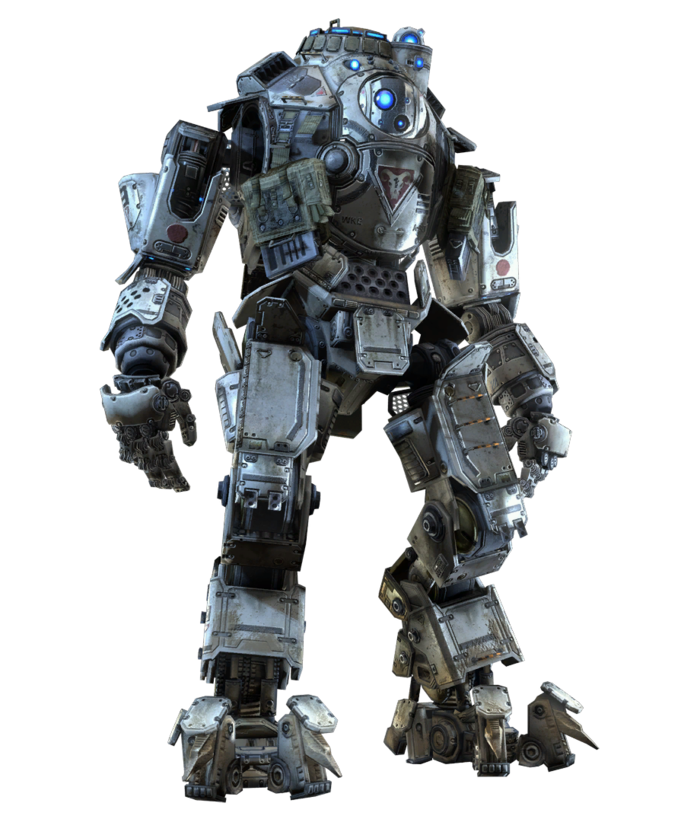
\includegraphics[width=\linewidth]{Atlas}
\end{wrapfigure}


The Atlas is the original Titan model produced by Hammond Robotics. It has a balance of mobility and armor, having more mobility than the Ogre, but more armor than the Stryder. This was the first Titan to be revealed.

The Atlas seems to be the second tallest Titan model, though exact measurements are unknown. Based on photos of the Atlas standing next to a pilot, it can be estimated to be between 20-25 feet tall. Its main entry point is in its chest, which opens up for the player. The Atlas also has a secondary entry point---a small hatch in the top. This is also the eject port for the Atlas.

The Atlas is the oldest Titan model on the Frontier and has instigated the development of both the Stryder and Ogre patterns. It was used through the Titan Wars, and onto the Frontier War. The Atlas is equipped with a Damage Core, which, when ready, the pilot can activate on command to substantially increase damage dealt by the titan.

\textbf{Damage Core}: The Atlas-class Titan has an in-built damage core. Once per round on your turn, you may cause the titan to suffer 1 system strain to perform the Aim maneuver as an Incidental.\\[1em]

\Vehicle{3}{2}{+0}{2}{2}{15}{15}

\begin{multicols}{2}
\noindent\textbf{Control Skill:} Pilot (Titan)\\
\noindent\textbf{Complement:} One pilot\\
\noindent\textbf{Passenger Capacity:} None\\
\noindent\textbf{Price/Rarity:} 21,750/8\\
\noindent\textbf{Consumables:} None\\
\noindent\textbf{Encumbrance Capacity:} 2\\
\noindent\textbf{Weapons:} Titan punch (Pilot [Titan]; Damage 2; Critical 3; Range [Engaged])\\
\noindent\textbf{Hard Points:} 3
\end{multicols}

\vspace*{\fill}
\pagebreak

\section{Ogre}
\label{sec:ogre}
\begin{wrapfigure}[12]{r}{.34\linewidth}
\vspace*{-2em}
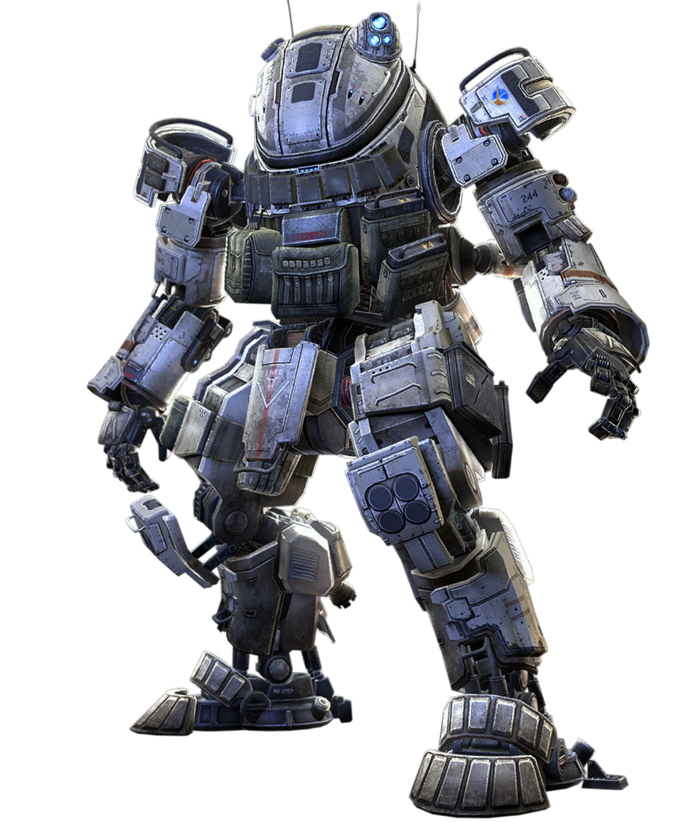
\includegraphics[width=\linewidth]{Ogre}
\end{wrapfigure}

The H-KA02/a Ogre Heavy Titan is a Titan model produced by Hammond Armament Division and Wonyeon Defense. Developed as an extremely tough Titan chassis, the Ogre's design has been compared to a main battle tank, optimized for taking higher amounts of damage and dealing out more than the Atlas or Stryder Titans. The Ogre stands slightly taller than the Atlas and has bulkier armor. The main entry point of an Ogre is via a large hatch on its top rather than the chest, like the Atlas or Stryder. The Ogre is equipped with a Shield Core, which amps the Titan's shield for a limited time.

\textbf{Shield Core}: The Ogre-class Titan has an in-built shield core. Once per round on your turn, you may cause the titan to suffer 1 system strain to perform the Brace for Impact maneuver as an Incidental.\\[3em]

\Vehicle{3}{1}{-2}{2}{2}{18}{18}


\begin{multicols}{2}
\noindent\textbf{Control Skill:} Pilot (Titan)\\
\noindent\textbf{Complement:} One pilot\\
\noindent\textbf{Passenger Capacity:} None\\
\noindent\textbf{Price/Rarity:} 25,740/8\\
\noindent\textbf{Consumables:} None\\
\noindent\textbf{Encumbrance Capacity:} 2\\
\noindent\textbf{Weapons:} Titan punch (Pilot [Titan]; Damage 2; Critical 3; Range [Engaged]; Vicious 1)\\
\noindent\textbf{Hard Points:} 3
\end{multicols}



No Titan is complete without its weapons. Most Titans have one primary, handheld weapon, one ordnance launcher and one defensive system. Some pilots prefer to change it up a bit and go for extra defense or offense. 

\section{Titan Weapons}

Each main weapon takes up one hard point on the Titan. Titan primary weapons follow the same rules as personal-scale weapons with regards to ammo. Unless you get an out of ammo result due to a \Despair\ (or \Threat\Threat\Threat\ for some weapons) the Titan is assumed to carry enough reloads to not worry about them.

Titan ordnance, on the other hand, has a limit to how much can be stored in a launcher at a time. Once all ammo is fired, that's it until the Titan can be rearmed at an appropriate facility. Note that you can install the Extra Ammo attachment to provide one reload for one installed ordnance weapon.

\subsection{40mm Cannon}

\begin{wrapfigure}[3]{l}{.34\linewidth}
\vspace*{-2em}
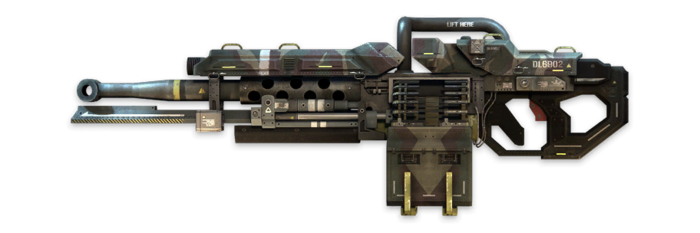
\includegraphics[width=\linewidth]{40mmCannon}
\end{wrapfigure}

The factory issue 40mm Cannon is a semi-automatic weapon that fires a high-explosive round with good accuracy. 

\subsection{Arc Cannon}
\begin{wrapfigure}[4]{r}{.34\linewidth}
\vspace*{-2em}
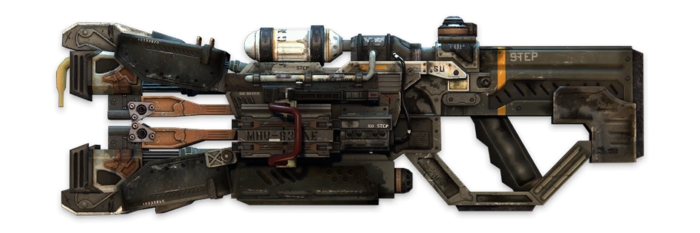
\includegraphics[width=\linewidth]{ArcCannon}
\end{wrapfigure}

The factory issue Arc Cannon fires a bolt of lightning that propagates across multiple targets. It can be fired quickly, or charged up over time for an increase in firepower. If you perform the Prepare maneuver, increase the damage of one hit of the next combat check by 1 and an arc cannon can negate Defense granted by energy shields by spending \Advantage\Advantage.

\subsection{PR-01 Plasma Railgun}
\begin{wrapfigure}[3]{l}{.34\linewidth}
\vspace*{-2em}
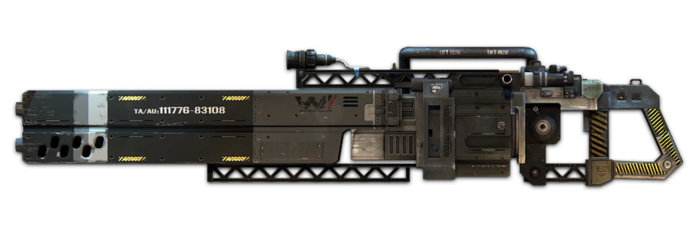
\includegraphics[width=\linewidth]{PlasmaRailgun}
\end{wrapfigure}

The Plasma Railgun is a Titan-sized sniper weapon, used for suppression of armored targets from a distance. The weapon fires a bolt of plasma, accelerated by a system of charged rails.


\subsection{Quad Rocket}
\begin{wrapfigure}[2]{r}{.34\linewidth}
\vspace*{-2em}
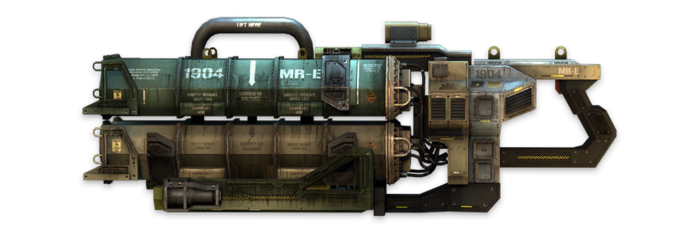
\includegraphics[width=\linewidth]{QuadRocket}
\end{wrapfigure}

The Quad Rocket is a weapon that fires a tight-knit cluster of 4 rockets at the target, exploding upon impact.

\subsection{Triple Threat}
\begin{wrapfigure}[4]{l}{.34\linewidth}
\vspace*{-2em}
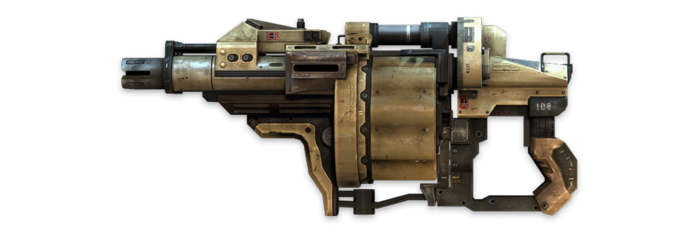
\includegraphics[width=\linewidth]{TripleThreat}
\end{wrapfigure}

The Triple Threat is a grenade launcher that shoots 3 grenades at once. It excels at clearing rooms, and its grenades explode on armored contact, making it effective at close range against other Titans. Due to the low magazine capacity, however, this weapon can run out of ammo by spending \Threat\Threat\Threat\ (instead of the normal \Despair).

\subsection{XOTBR-16 Chaingun}
\begin{wrapfigure}[3]{r}{.34\linewidth}
\vspace*{-2em}
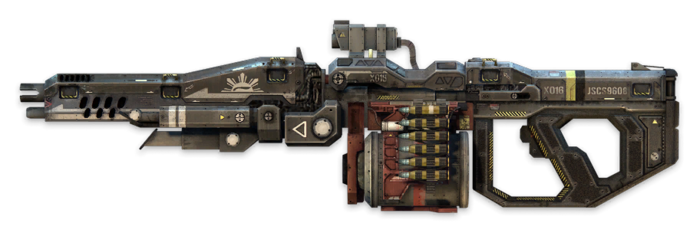
\includegraphics[width=\linewidth]{XO16Chaingun}
\end{wrapfigure}

The XO-16 Chaingun is a fully automatic ballistic weapon that fires 1.6 inch slugs with high precision at considerable range.

\begin{table}[h!]
\caption{Titan Weapons}
\footnotesize
\begin{GenesysTable}{*{2}{l} *{2}{c} l c r c X[l]}
Name & Skill & Dam & Crit & Range  & HP & Price & Rarity & Special\\
40mm Cannon & Gunnery & 6 & 3 & Long & 1 & 7,750 & 6 & Blast 1, Breach 1 \\
Arc Cannon & Gunnery & 4 & 4 & Medium & 1 & 5,250 & 7 & Blast 3, Special\\
Plasma Railgun & Gunnery & 7 & 2 & Extreme & 1 & 10,750 & 7 & \Special{Accurate 1, Breach 1, Limited Ammo 2}
Quad Rocket & Gunnery & 4 & 3 & Long & 1 & 7,500 & 6 & \Special{Accurate 1, Blast 3, Vicious 2}
Triple Threat & Gunnery & 4 & 4 & Medium & 1 & 8,250 & 7 & \Special{Blast 2, Linked 2, Special}
XO-16 Chaingun & Gunnery & 3 & 4 & Long & 1 & 4,750 & 7 & Auto-fire
\end{GenesysTable}
\end{table}

\section{Titan Ordnance}
Unless otherwise noted, extra reloads for ordnance weapons cost 2,000 credits.

\subsection{Cluster Missile}
\begin{wrapfigure}[4]{l}{.34\linewidth}
\vspace*{-2em}
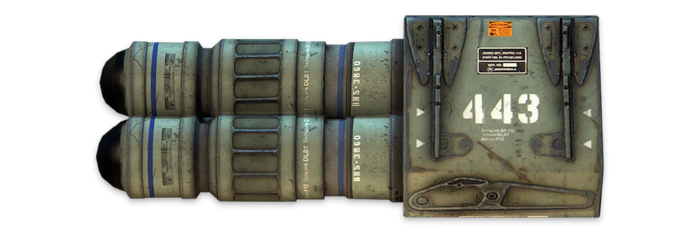
\includegraphics[width=\linewidth]{ClusterMissile}
\end{wrapfigure}

The Cluster Missile pod fires a missile which, on impact, deploys a shower of secondary explosive charges that continue to explode and saturate an area for a considerable time.

\subsection{Laser Shot}
The laser shot fires a lethal beam that cuts through anything in its way. It's a directed energy weapon that takes the charge rifle and and amps it up to Titan-scale.

\subsection{Multi-Target Missile System}
\begin{wrapfigure}[3]{r}{.34\linewidth}
\vspace*{-2em}
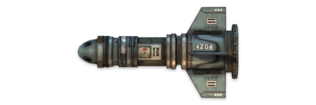
\includegraphics[width=\linewidth]{MultiTargetMissileSystem}
\end{wrapfigure}

The Multi-Target Missile System enables you to engage multiple targets at once. The Guided quality can only be activated when attacking targets made of significant metal content, like Titans and Spectres.

\subsection{Rocket Salvo}
\begin{wrapfigure}[2]{l}{.34\linewidth}
\vspace*{-2em}
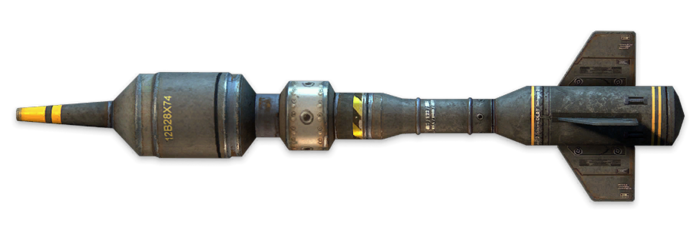
\includegraphics[width=\linewidth]{RocketSalvo}
\end{wrapfigure}

The Rocket Salvo launches a rapid salvo of unguided rockets. Each \Success\  deals +2 damage, instead of +1.

\subsection{Slaved Warheads}
\begin{wrapfigure}[3]{r}{.34\linewidth}
\vspace*{-2em}
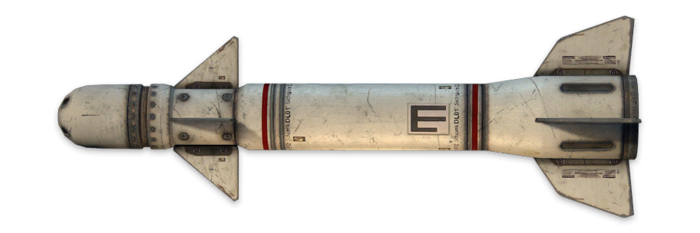
\includegraphics[width=\linewidth]{SlavedWarheads}
\end{wrapfigure}

This Titan ordnance pod requires a lock-on before you can fire. When you fire, a barrage of 3 homing missiles will launch towards your locked target. The Guided quality can only be activated when attacking targets made of significant metal content, like Titans and Spectres.


\begin{table}[h!]
\caption{Titan Ordnance}
\footnotesize
\begin{GenesysTable}{*{2}{l} *{2}{c} l c r c X[l]}
Name & Skill & Dam & Crit & Range  & HP & Price & Rarity & Special\\
Cluster Missile & Gunnery & 4 & 3 & Extreme & 1 & 6,250 & 8 & \Special{Blast 4, Breach 1, Limited Ammo 3}
Laser Shot & Gunnery & 3 & 2 & Long & 1 & 5,100 & 8 & \Special{Accurate 1, Breach 2, Slow-Firing 1, Vicious 2}
MTM System & Gunnery & 5 & 3 & Extreme & 1 & 9,000 & 8 & \Special{Accurate 1, Auto-Fire, Breach 1, Guided 3, Limited Ammo 3, Special}
Rocket Salvo & Gunnery & 3 & 2 & Long & 1 & 7,050 & 8 & \Special{Blast 1, Breach 2, Inaccurate 1, Limited Ammo 2, Special}
Slave Warhead & Gunnery & 5 & 4 & Long & 1 & 8,250 & 8 & \Special{Blast 1, Breach 1, Guided 2, Limited Ammo 3, Linked 2}
\end{GenesysTable}
\end{table}


\section{Defensive Systems}
Titans are not indestructible, regardless of what the IMC wants you to believe. Each Titan is equipped with one of three defensive systems, designed to prolong the lifespan of the Titan.


\subsection{Electric Smoke}
\begin{wrapfigure}[6]{l}{.25\linewidth}
\vspace*{-2em}

\includegraphics[width=\linewidth]{ElectricSmoke}
\end{wrapfigure}

Electric smoke is a reactionary device used to avoid attacks and negate tracking weapons.

Once per round, as an out-of-turn incidental, you may deploy a smoke charge. If this was done as a reaction to being targeted by a Guided weapon, the tracking is lost and the weapon may not fire on your Titan this turn. It creates an area of obscurant around your Titan that grants concealment worth +3 dice (see page 110 of the \emph{Genesys} Core Rulebook).Any pilot on your Titan must immediately move away from your Titan or risk taking damage from the electric smoke. If they won't (or can't) disembark, they must make a \textbf{Hard (\DifficultyDie\DifficultyDie\DifficultyDie) Resilience check} or suffer 1 wound, plus 1 additional wound per \Failure. If the Resilience check generates \Threat\Threat, they become Disoriented for two rounds. This cloud lasts until the end of your next turn. Any pilot that ends their turn in the smoke must make the Resilience check or suffer wound as described above.

If the skill check that triggered the electric smoke generates \Advantage\Advantage, it may be spent to cause you to have only one smoke canister left.

\subsection{Partical Wall}
\begin{wrapfigure}[6]{r}{.25\linewidth}
\vspace*{-4em}

\includegraphics[width=\linewidth]{ParticleWall}
\end{wrapfigure}

The particle wall creates a concave force field which blocks all projectiles from one side and lets all projectiles through from the other. As an incidental you may deploy the particle wall in front of your Titan. It grants Ranged Defense 4 to all Titans behind the wall. It lasts until the end of your next turn, and it requires two rounds to recharge before it can be used again.

\subsection{Vortex Shield}
\begin{wrapfigure}[7]{l}{.25\linewidth}
\vspace*{-2em}

\includegraphics[width=\linewidth]{VortexShield}
\end{wrapfigure}

The Vortex Shield allows Titans to stop enemy fire such as rockets and bullets in their tracks and is able to send the projectiles right back to the enemy.

As an out-of-turn incidental you may deploy the vortex shield when targeted by a ranged combat check. It provides the Reflective 1 quality until the beginning of your next turn. If the triggering attack generates \Threat\Threat\Threat, you may reflect the projectile (if any) back on the target, dealing the weapon's base damage to the attacker. If the check generates \Despair, you instead deal a Critical Injury (or a Critical Hit for vehicles).

\begin{table}[h!]
\centering
\caption{Titan Defensive Systems}
\footnotesize
\begin{GenesysTable}{*{2}{l} *{2}{c} l c r c X[l]}
System & Hard Point & Price & Rarity\\
Electric Smoke & 1 & 2,000 & 8\\
Particle Wall & 1 & 3,000 & 8\\
Vortex Shield & 1 & 1,000 & 8
\end{GenesysTable}
\end{table}

%%%%%
% Appendices
%%%%%

\appendix

\chapter{Change Log}
\label{changelog}
{\small

\section{June 2018}

\subsection{v0.7.2---7.June}
\begin{itemize}[noitemsep]
\item Added Stim and grapple as armour attachments
\item Added cloak as an armour
\item Data knife item changed to dataspike weapon attachment
\item Custom weapon attachments added
\item Custom armour attachments added
\item Heavy jacket's HP removed, price lowered
\item Panacea added to gear section
\end{itemize}


\subsection{v0.7.1--5.Jun}
\begin{itemize}[noitemsep]
\item Fixed DMR and kraber limited ammo wonkiness
\item Clarified how Titan weapon ammo works
\item Changed encrypted comm-bead's price
\end{itemize}

\section{May 2018}

\subsection{v0.7--29.May}
\begin{itemize}[noitemsep]
\item Changed encrypted comm-bead mechanics
\item Added firestar
\item Added pulse blade
\item Added pilot electric smoke
\item Reworked weapon prices
\item Added Titan defense systems
\end{itemize}

\subsection{v0.6---25.May}
\begin{itemize}[noitemsep]
\item Added armour section
\item Added gear section
\item Added attachment chapter
\item Listed GCRB attachments available
\item Welcome to the Militia intro chapter added
\end{itemize}

\subsection{v0.5---23.May}
\begin{itemize}[noitemsep]
\item Cover page art
\item Titan ordnance table added
\item Added spacing around `Special' column in weapon tables
\end{itemize}

\subsection{v0.4---22.May}
\begin{itemize}[noitemsep]
\item Titan weapon table added
\item Titan ordnance descriptions added
\item ToC added
\end{itemize}


\subsection{v0.3---20.May}
\begin{itemize}[noitemsep]
\item Archer damage and blast increased
\item Mag launcher range reduced
\item Sidewinder damage increased
\item Made charge rifle a crit fishing weapon
\item Added Titan weapons descriptions
\end{itemize}


\subsection{v0.2---19.May}
\begin{itemize}[noitemsep]
\item Changed LMG skill to Gunnery
\item Increased EVA-8's blast from 4 to 6
\item Anti-Titan weapons added
\item Pilot ordnance added
\end{itemize}


\subsection{v0.1---14.May}
\textbf{Initial Compilation}

\begin{itemize}[noitemsep]
\item Stryder-class titan added
\item Atlas-class titan added
\item Ogre-class titan added
\item Sidearms added
\item Longarms added
\end{itemize}


}

















\end{document}
